%!TEX root = ../../../thesis.tex
This section contains supplementary data to the measurements made in \cref{chap:fluid_mimicry}.
It details some of the testing done to ensure that the measurement setup was providing expected results, and test the electrodes for defects.
It also contains measurements not presented in the thesis body.
They have been included purely for interests sake.


\begin{figure}
    \centering
    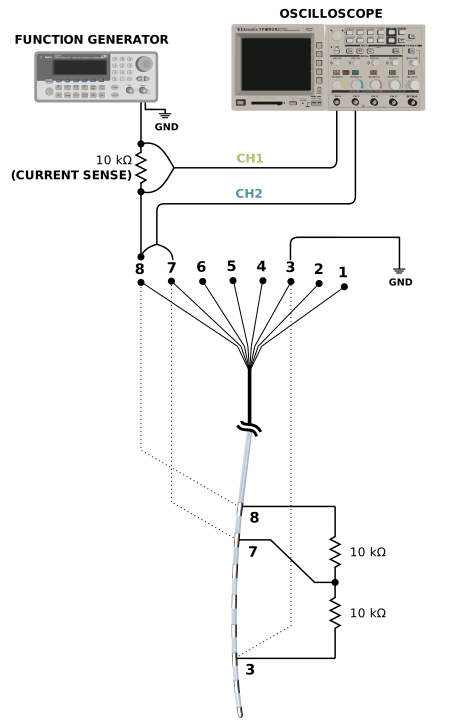
\includegraphics[scale=0.95]{content/appendices/Solution-Impedance-Measurements/graphics/Solution-Impedance-Testing-Setup}
    \caption{\label{fig:solution_impedance_testing_setup}Diagram showing the instruments and electrode configuration used to test the measurement setup.}
\end{figure}

Due to the impedance drop at low frequencies that was encountered when measuring the various solutions presented in \cref{chap:fluid_mimicry}, some testing of the measurement setup was done.
\Cref{fig:solution_impedance_testing_setup} shows the configuration used to test the electrode.
The electrodes were included to determine whether they themselves were contributing to the impedance magnitude drop at low frequency.


\begin{figure}
    \centering
    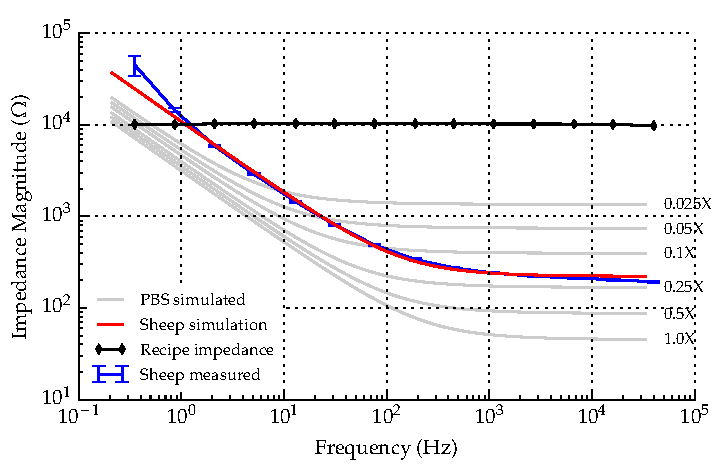
\includegraphics{content/appendices/Solution-Impedance-Measurements/graphics/run14_calibration_10k_noWater_ZVsF_graph_mag}
    \caption{\label{fig:calibration_10kRes_mag}Graph of impedance magnitude versus frequency (log-log) for a \SI{10}{\kilo\ohm} resistor placed between electrodes one and two, and another \SI{10}{\kilo\ohm} resistor placed between electrodes two and five.}
\end{figure}

\begin{figure}
    \centering
    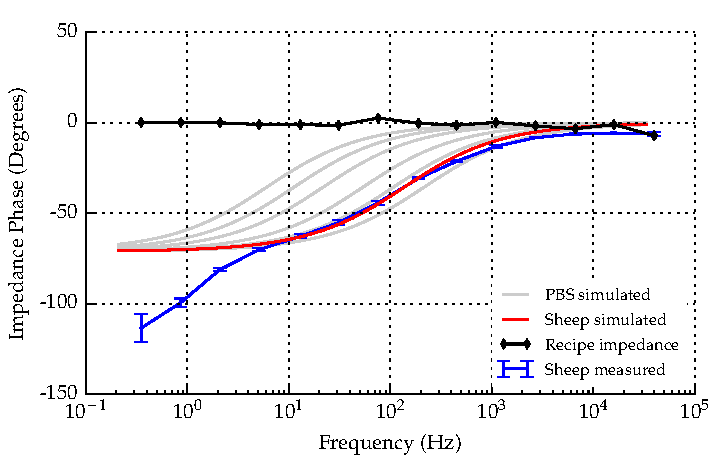
\includegraphics{content/appendices/Solution-Impedance-Measurements/graphics/run14_calibration_10k_noWater_ZVsF_graph_phase}
    \caption{\label{fig:calibration_10kRes_phase}Graph of impedance phase versus frequency (log-log) for a \SI{10}{\kilo\ohm} resistor placed between electrodes one and two, and another \SI{10}{\kilo\ohm} resistor placed between electrodes two and five.}
\end{figure}

\Cref{fig:calibration_10kRes_mag,fig:calibration_10kRes_phase} show that the measurement setup \emph{is} capable of measuring a target \SI{10}{\kilo\ohm} resistance placed between electrode one and two.
These measurements include the electrode array in the loop so any effect from the internal wiring will be evident here.


\begin{figure}
    \centering
    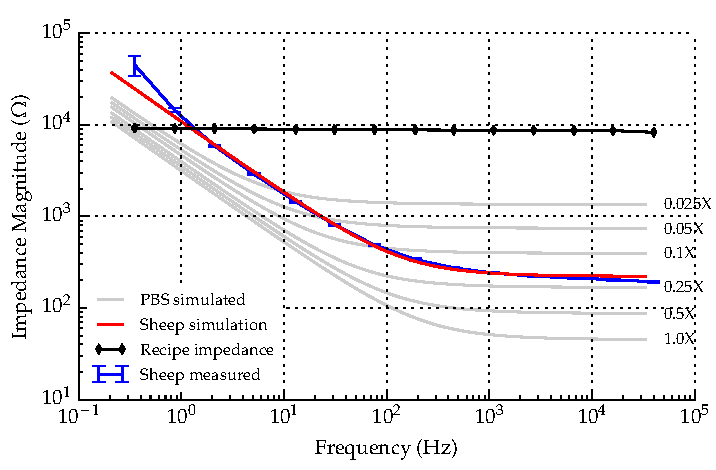
\includegraphics[width=\textwidth]{content/appendices/Solution-Impedance-Measurements/graphics/run14_calibration_10k_water_ZVsF_graph_mag}
    \caption{\label{fig:calibration_10kRes_water_mag}Graph of impedance magnitude versus frequency (log-log) for a \SI{10}{\kilo\ohm} resistor placed between electrodes one and two, and another \SI{10}{\kilo\ohm} resistor placed between electrodes two and five. The electrodes and resistors are submerged in distilled water.}
\end{figure}

\begin{figure}
    \centering
    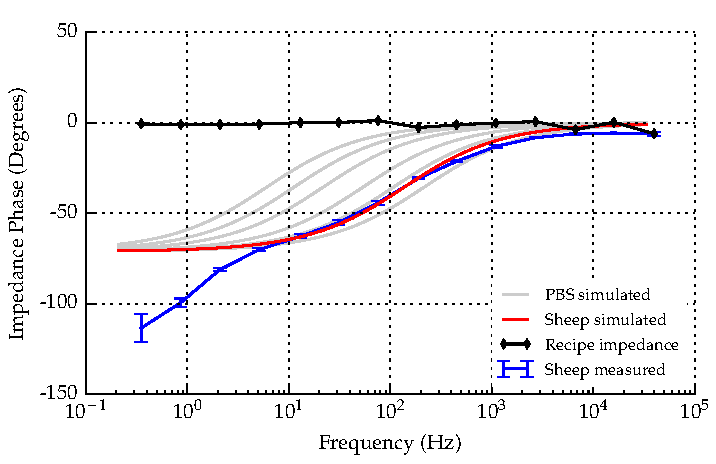
\includegraphics[width=\textwidth]{content/appendices/Solution-Impedance-Measurements/graphics/run14_calibration_10k_water_ZVsF_graph_phase}
    \caption{\label{fig:calibration_10kRes_water_phase}Graph of impedance phase versus frequency (log-log) for a \SI{10}{\kilo\ohm} resistor placed between electrodes one and two, and another \SI{10}{\kilo\ohm} resistor placed between electrodes two and five. The electrodes and resistors are submerged in distilled water.}
\end{figure}

\Cref{fig:calibration_10kRes_water_mag,fig:calibration_10kRes_water_phase} show the effect of submerging the electrode array in liquid. The resistors from the previous test are still in place, and therefore are also submerged.
The resistance has dropped slightly, as expected, but no impedance deviation at low frequency is evident.
This rules out the possibility of a wet electrode array having an effect on the measurement results due to leakage.

\begin{figure}
    \centering
    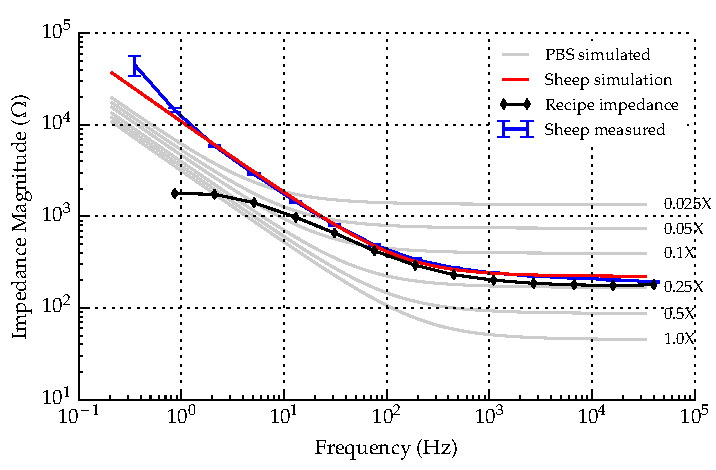
\includegraphics[width=\textwidth]{content/appendices/Solution-Impedance-Measurements/graphics/run14_calibration_10k_water_salt_amended_ZVsF_graph_mag}
    \caption{\label{fig:calibration_10kRes_saline_mag}Graph of impedance magnitude versus frequency (log-log) for a \SI{10}{\kilo\ohm} resistor placed between electrodes one and two, and another \SI{10}{\kilo\ohm} resistor placed between electrodes two and five. The electrodes and resistors are submerged in saline.}
\end{figure}

\begin{figure}
    \centering
    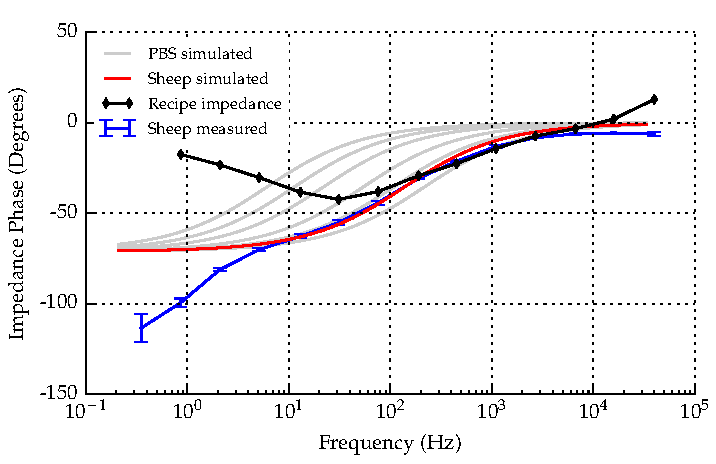
\includegraphics[width=\textwidth]{content/appendices/Solution-Impedance-Measurements/graphics/run14_calibration_10k_water_salt_amended_ZVsF_graph_phase}
    \caption{\label{fig:calibration_10kRes_saline_phase}Graph of impedance phase versus frequency (log-log) for a \SI{10}{\kilo\ohm} resistor placed between electrodes one and two, and another \SI{10}{\kilo\ohm} resistor placed between electrodes two and five. The electrodes and resistors are submerged in saline.}
\end{figure}

\Cref{fig:calibration_10kRes_saline_mag,fig:calibration_10kRes_saline_phase} shows the effect of adding salt to the solution.
That the characteristic impedance drop at low frequencies is evident.
This result adds weight to the theory that it is ions in the solution that is responsible for the impedance magnitude drop at low frequency.
